\documentclass{article}

\usepackage[T1]{fontenc}
\usepackage{siunitx}
\usepackage[polish]{babel}
\usepackage[utf8]{inputenc}
\usepackage{float}
\usepackage{graphicx}
\usepackage{amsmath}
\usepackage{siunitx}
\usepackage{longtable}
\oddsidemargin 0pt
\evensidemargin 0pt
\marginparwidth 40pt
\marginparsep 10pt
\topmargin -20pt
\headsep 10pt
\textheight 8.7in
\textwidth 6.65in
\linespread{1.2}

\title{Sprawozdanie z Laboratorium 5.}
\author{Piotr Lewandowski \and Dymitr Lubczyk \and Krzysztof Tabeau }
\date{\today}
\begin{document}
\maketitle
\subsection{Informacje}
\begin{tabular}{|l|l|}
\hline
Autorzy             & Dymitr Lubczyk                    \\
                    & Krzysztof Tabeau                  \\
                    & Piotr Lewandowski                 \\
Wydział             & Matematyki i Nauk Informacyjnych  \\
Numer Zespołu       & 19                                \\
Data laboratorium   & 17:15 08.06.2020                  \\
Numer laboratorium  & 5                                 \\
Prowadzący          & dr inż. Kamil Orzechowski         \\
\hline
\end{tabular}
\subsection{Tytuł ćwiczenia}
Pomiar długości fal elektromagnetycznych metodami interferencyjnymi
\subsection{Cel ćwiczenia}
Celem ćwiczenia jest wyznaczenie długości fal elektromagnetycznych metodami interferencyjnymi, w tym interferometrem Michelsona, siatką dyfrakcyjną oraz dwuwymiarową siecią dyfrakcyjną.
\clearpage

\section{Część teoretyczna}

\subsection{Wstęp}
W poniższym sprawozdaniu opiszemy nasze doświadczenia z różnymi metodami wyznaczania długości fal elektromagnetycznych za pomocą zjawiska interferencji fal i ich wyniki. Wykorzystamy do tego interferometr Michelsona, siatkę dyfrakcyjną i dwuwymiarową sieć dyfrakcyjną. W jaki sposób możemy otrzymać wynik używając tych układów, zostanie zawarte wraz z opisem układu. Zanim jednak do tego przejdziemy wyjaśnimy pojęcia, które pojawią się dalej.

\begin{itemize}
\item Fala elektromagnetyczna - zaburzenie pola elektromagnetycznego
\item Dyfrakcja - zjawisko ugięcia światła wokół krawędzi przeszkody lub otworu w obszarze cienia przeszkody.
\item Interferencja - efekt nakładania się fal. Może skutkować wzmocnieniem lub osłabieniem natężenia fali wypadkowej.
\end{itemize}

\subsection{Opis układów doświadczalnych}

\subsubsection{Interferometr Michelsona}
Klasycznie urządzenie wykorzystuje dwa zwierciadła, półprzezroczystą płytkę i oczywiście źródło i detektor fal elektromagnetycznych. Podczas naszego doświadczenia, jako źródło fal został użyty laser, a jako detektor zwykły aparat podłączony do tabletu. Dodatkowo została użyta pinhola dla lepszej kontroli miejsca padania lasera. \\
Interferometr działa w następujący sposób. Wiązka pada na półprzezroczystą płytkę, która przepuszcza połowę natężenia fali, a drugą odbija do zwierciadła, które z kolei odbija ją do detektora. Przepuszczona połowa pada również na zwierciadło, które odbija je z powrotem na płytkę, która odbija ją do detektora. \\
Aby wyznaczyć długość fali trzeba odpowiednio manipulować odległościami zwierciadła od płytki, co przekłada się na przesuniecie się prążków interferencyjnych na detektorze. Jeśli uda się przesunąć zwierciadło tak, aby z maksymalnego wzmocnienia przejść do drugiego maksymalnego wzmocnienia to wiemy, że przesunęliśmy zwiększyliśmy lub zmniejszyliśmy drogę fali i o jedną jej długość. w ten sposób powstaje poniższy wzór, gdzie \textit{$\lambda$} to długość fali, \textit{$\delta$} to dystans przesuniętego zwierciadła, a \textit{m} to liczba odpowiadająca kolejnym zmianom maksymalnych wzmocnień obserwowanych na detektorze.
\begin{gather*}
     \lambda = \frac{2\delta}{m}
\end{gather*}

\subsubsection{Siatka dyfrakcyjna}
Jest to przyrząd z wąskimi równoległymi szczelinami zamieszczonymi blisko siebie. Fala elektromagnetyczna przechodząca przez siatkę ulega dyfrakcji, czyli każde szczelina staje się osobnym źródłem fali. Następnie fale interferują ze sobą tworząc na powierzchni za siatką prążki interferencyjne. \\
Na podstawie odległości powierzchni za siatką od siatki (\textit{L}), odległości między środkami szczelinami (\textit{d}) i odległości między środkami prążków (\textit{$H_{m}$}), można wyznaczyć długość fali za pomocą poniższych wzorów, gdzie \textit{m} to numer prążka.
\begin{gather*}
    \tan\Theta = \frac{H_{m}}{L} \\
    \lambda = \frac{d\sin\Theta}{m}
\end{gather*}

\subsubsection{Dwuwymiarowa sieć dyfrakcyjna}
Jak sama nazwa wskazuje, jest to urządzenie zbliżone do siatki dyfrakcyjnej, tylko że zamiast wąskich szczelin występują tutaj małe prostokątne dziurki. W wyniku zamiast prążków na płaszczyźnie za siecią pojawią się zbliżone prostokątowi figury.\\
Do wyznaczenia długości fali będziemy potrzebować dwóch prostokątów wynikowych, które potem będziemy nazywać prostokątem bazowym i prostokątem przyrównywanym.
Oznaczymy szerokość dziurki jako \textit{$\xi$}, a wysokość jako \textit{$\eta$}. Oznaczmy \textit{k}, jako numer wiersza prostokąta przyrównywanego, względem prostokąta bazowego, a \textit{h} analogicznie kolumną. 
Dodatkowo niech \textit{$H_{hk}$} będzie odległością między porównywanymi prostokątami, a L odległością powierzchnią za siecią od sieci.
Niech m będzie liczbą naturalną.
\begin{gather*}
    \tan(\Theta_{hk}) = \frac{H_{hk}}{L} \\
    d_{hk} = \frac{1}{\sqrt{\frac{h^2}{\xi^2}+\frac{k^2}{\eta^2}}} \\
    \lambda = \frac{d_{hk}\sin(\Theta_{hk})}{m}
\end{gather*}

\clearpage
\section{Część doświadczalna}
\subsection{Wykonane pomiary}
\subsubsection{Pomiary z interferometru Michelson'a}
\begin{table}[h!]
\tiny
\centering
\begin{tabular}{|l|l|l|l|l|l|}
\hline
Pozycja suwaka & Natężenie światła & Pozycja suwaka & Natężenie światła	&	Pozycja suwaka & Natężenie światła\\ \hline
0	&	255	&	6.67	&	2	&	13.54	&	30	\\
0.21	&	75	&	6.77	&	81	&	13.64	&	6	\\
0.31	&	1	&	6.87	&	204	&	13.74	&	98	\\
0.41	&	47	&	6.97	&	254	&	13.85	&	217	\\
0.51	&	170	&	7.08	&	184	&	13.95	&	251	\\
0.62	&	252	&	7.18	&	60	&	14.05	&	168	\\
0.72	&	216	&	7.28	&	0	&	14.15	&	46	\\
0.82	&	95	&	7.38	&	61	&	14.26	&	1	\\
0.92	&	6	&	7.49	&	186	&	14.36	&	77	\\
1.03	&	32	&	7.59	&	254	&	14.46	&	200	\\
1.13	&	149	&	7.69	&	202	&	14.67	&	188	\\
1.23	&	245	&	7.79	&	79	&	14.77	&	64	\\
1.33	&	230	&	7.9	&	2	&	14.87	&	0	\\
1.44	&	117	&	8	&	44	&	14.97	&	57	\\
1.54	&	14	&	8.1	&	165	&	15.08	&	181	\\
1.74	&	127	&	8.21	&	251	&	15.18	&	254	\\
1.85	&	235	&	8.31	&	219	&	15.28	&	206	\\
1.95	&	242	&	8.41	&	100	&	15.38	&	84	\\
2.05	&	139	&	8.51	&	7	&	15.49	&	3	\\
2.15	&	26	&	8.62	&	28	&	15.59	&	40	\\
2.26	&	9	&	8.82	&	244	&	15.69	&	161	\\
2.36	&	105	&	8.92	&	233	&	15.79	&	249	\\
2.46	&	222	&	9.03	&	122	&	15.9	&	222	\\
2.56	&	250	&	9.13	&	16	&	16	&	105	\\
2.67	&	161	&	9.23	&	16	&	16.1	&	9	\\
2.77	&	40	&	9.33	&	122	&	16.21	&	25	\\
2.87	&	3	&	9.44	&	233	&	16.31	&	139	\\
2.97	&	84	&	9.54	&	244	&	16.41	&	241	\\
3.08	&	206	&	9.64	&	144	&	16.51	&	236	\\
3.18	&	254	&	9.74	&	29	&	16.62	&	127	\\
3.28	&	181	&	9.85	&	7	&	16.72	&	19	\\
3.38	&	58	&	9.95	&	100	&	16.82	&	14	\\
3.49	&	0	&	10.05	&	219	&	16.92	&	117	\\
3.59	&	64	&	10.15	&	251	&	17.03	&	230	\\
3.69	&	188	&	10.36	&	44	&	17.13	&	245	\\
3.79	&	255	&	10.46	&	2	&	17.23	&	149	\\
3.9	&	200	&	10.56	&	79	&	17.33	&	32	\\
4	&	77	&	10.67	&	202	&	17.44	&	6	\\
4.1	&	1	&	10.77	&	254	&	17.54	&	95	\\
4.21	&	46	&	10.87	&	186	&	17.64	&	215	\\
4.31	&	168	&	10.97	&	62	&	17.74	&	252	\\
4.41	&	251	&	11.08	&	0	&	17.85	&	170	\\
4.51	&	217	&	11.18	&	59	&	17.95	&	48	\\
4.62	&	98	&	11.28	&	183	&	18.05	&	1	\\
4.72	&	6	&	11.38	&	254	&	18.15	&	74	\\
4.82	&	30	&	11.49	&	204	&	18.26	&	198	\\
4.92	&	146	&	11.59	&	81	&	18.46	&	190	\\
5.03	&	244	&	11.79	&	42	&	18.56	&	66	\\
5.13	&	231	&	11.9	&	163	&	18.67	&	0	\\
5.23	&	120	&	12	&	250	&	18.77	&	55	\\
5.33	&	15	&	12.1	&	221	&	18.87	&	179	\\
5.44	&	17	&	12.21	&	103	&	18.97	&	254	\\
5.54	&	124	&	12.31	&	8	&	19.08	&	208	\\
5.64	&	234	&	12.41	&	27	&	19.18	&	86	\\
5.74	&	243	&	12.51	&	141	&	19.28	&	3	\\
5.85	&	142	&	12.62	&	242	&	19.38	&	38	\\
5.95	&	27	&	12.72	&	234	&	19.49	&	158	\\
6.05	&	8	&	12.92	&	17	&	19.59	&	249	\\
6.15	&	102	&	13.03	&	15	&	19.69	&	224	\\
6.26	&	221	&	13.13	&	119	&	19.79	&	107	\\
6.36	&	250	&	13.23	&	231	&	19.9	&	10	\\
6.46	&	163	&	13.33	&	245	&	20	&	24	\\
6.56	&	42	&	13.44	&	146	&		&		\\
\hline
\end{tabular}
\end{table}
Pomiarów jest dużo, ale dzięki temu uzyskamy lepsze rezultaty. Jak można też zauważyć na pierwszy rzut oka to wyniki wyglądają sinusoidalnie. Wartość pozycji suwaka jest w mikrometrach, licząc od pozycji startowej, a natężenie światła w luksach.
\subsection{Pomiary siatki dyfrakcyjnej}
Aby skorzystać ze wzoru wspomnianego w punkcie 1.2.2 musimy w pierwszej kolejności wyznaczyć stałą siatki d, w tym celu przeanalizowaliśmy zdjęcia zamieszczone w załączniku do zadania. Po analizie pierwszego zdjęcia okazało się, że środki otworów występują średnio co 105 pixel, zaś po analizie zdjęcia wyznaczającego skalę zdjęcia okazało się, że 1 pixel odpowiada \SI{8,405}{\micro\metre}, co ostatecznie prowadzi do wyznaczenia odległości między środkami otworów:
\begin{equation}
    d=\SI{0.088}{\milli\metre}
\end{equation}
Poniższe wyniki zostały uzyskane dla L=580mm i przy założeniu, że 85 pixeli to jeden milimetr
\begin{table}[h!]
\centering
\begin{tabular}{|l|l|l|l|}
\hline
$m$ & $H[mm]$ & $sin\Theta$ & $\lambda[nm]$ \\ \hline
1 & 2.85 & 0.0049 & 435.8 \\
1 & 2.80 & 0.0048 & 428.6 \\
2 & 5.51 & 0.0095 & 421.4 \\
2 & 5.49 & 0.0095 & 420.5 \\
3 & 7.02 & 0.0121 & 358.3 \\
3 & 7.06 & 0.0122 & 360.1 \\
\hline
\end{tabular}
\caption{Wyniki dla światła fioletowego}
\end{table}
\begin{table}[h!]
\centering
\begin{tabular}{|l|l|l|l|}
\hline
$m$ & $H[mm]$ & $sin\Theta$ & $\lambda[nm]$ \\ \hline
1 & 3.65 & 0.0063 & 558.2 \\
1 & 3.53 & 0.0061 & 540.2 \\
2 & 7.26 & 0.0125 & 555.5 \\
2 & 7.29 & 0.0126 & 558.2 \\
3 & 10.74 & 0.0185 & 547.9 \\
3 & 10.99 & 0.0189 & 560.5 \\
\hline
\end{tabular}
\caption{Wyniki dla światła zielonego}
\end{table}

\begin{table}[h!]
\centering
\begin{tabular}{|l|l|l|l|}
\hline
$m$ & $H[mm]$ & $sin\Theta$ & $\lambda[nm]$ \\ \hline
1 & 4.36 & 0.0075 & 668.1 \\
1 & 4.36 & 0.0075 & 668.1 \\
2 & 8.87 & 0.0153 & 678.8 \\
2 & 8.89 & 0.0153 & 680.6 \\
\hline
\end{tabular}
\caption{Wyniki dla światła czerwonego}
\end{table}
\clearpage

\subsection{Pomiary dwuwymiarowej sieci dyfrakcyjnej}
Pomiary rozpoczynamy od wyznaczenia skali opracowywanych zdjęć, mierząc szerokość pixela. Dla zdjęcia linijki otrzymaliśmy 985.6 pixeli na 1 cm, co oznacza, że jeden pixel to 0.0101 mm. Dla zdjęcia siatki jest to średnio 676.6 pixeli na 1 mm, więc jeden pixel to 0.00148 mm.
\begin{table}[h!]
\centering
\begin{tabular}{|l|l|}
\hline
Linijka [pixel/cm] & Siatka [pixel/mm] \\ \hline
992 & 677 \\
980 & 677 \\
984 & 675 \\
992 & 677 \\
980 & 677 \\ \hline
\end{tabular}
\caption{Pomiary skali}
\end{table}

Kolejnym krokiem jest wyznaczenie parametrów $\xi$ oraz $\eta$ charakteryzujących wykorzystaną sieć dyfrakcyjną, które zgodnie z poniższymi wynikami wynoszą odpowiednio 68.2 pixeli (0.1008 mm) oraz 62.8 pixeli (0.0928 mm). Sieć została umieszczona w odległości L=580 mm od ekranu.
\begin{table}[h!]
\centering
\begin{tabular}{|l|l|}
\hline
$\xi$ [pixel] & $\eta$ [pixel] \\ \hline
65                   & 62 \\
66                   & 65 \\
68                   & 64 \\
70                   & 61 \\
72                   & 62 \\ \hline
\end{tabular}
\caption{Wyniki pomiarów sieci dyfrakcyjnej w pixelach}
\end{table}

Następnie możliwe jest zmierzenie wartości $H_{h,k}$, dla każdego ze zdjęć, wszystkie wartości zostały podane w milimetrach.
\begin{table}[H]
\centering
\begin{tabular}{r|rrr}
\multicolumn{1}{l|}{} & -1          & 0           & 1           \\ \hline
-1                    & 10.658 & 8.280 & 6.081 \\
0                     & 2.384  & 0.000 & 2.376 \\
1                     & 10.140 & 7.955 & 5.680
\end{tabular}
\caption{Pomiary $H_{h,k}$ dla koloru niebieskiego}
\end{table}

\begin{table}[H]
\centering
\begin{tabular}{r|rrr}
\multicolumn{1}{l|}{} & -1          & 0           & 1           \\ \hline
-1                    & 4.021  & 2.981 & 4.326 \\
0                     & 3.173  & 0.000 & 3.117 \\
1                     & 4.577  & 3.223 & 4.405 
\end{tabular}
\caption{Pomiary $H_{h,k}$ dla koloru zielonego}
\end{table}

\begin{table}[H]
\centering
\begin{tabular}{r|rrr}
\multicolumn{1}{l|}{} & -1          & 0           & 1           \\ \hline
-1                    & 5.367  & 3.902 & 5.080 \\
0                     & 3.923  & 0.000 & 3.754 \\
1                     & 5.801  & 3.964 & 5.417
\end{tabular}
\caption{Pomiary $H_{h,k}$ dla koloru czerwonego}
\end{table}

\clearpage



\section{Opracowanie wyników}
\subsection{Charakterystyka I(r)}
\begin{figure}[H]
\centerline{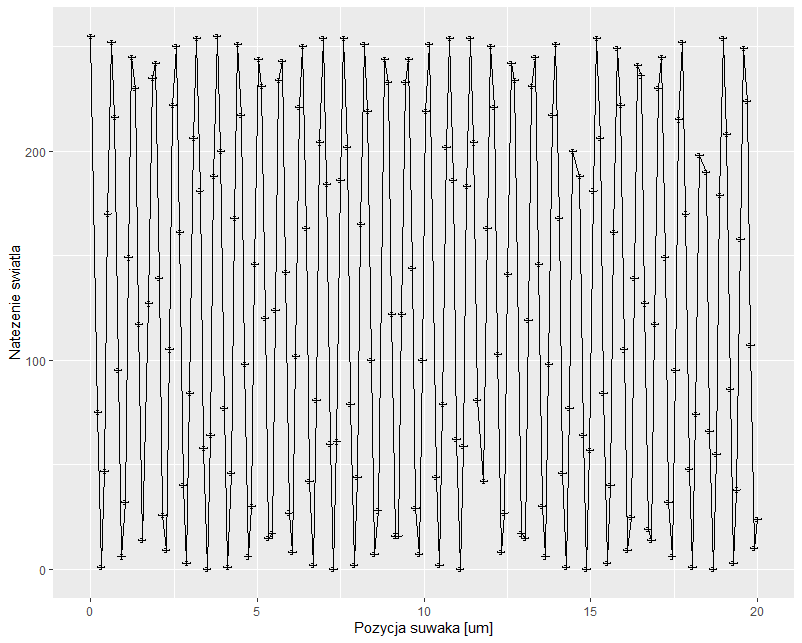
\includegraphics[scale=0.8]{Rplot.png}}
\end{figure}
Na powyższym wykresie zostały zobrazowane pomiary wraz z niepewnościami.
Z pomiarów możemy zauważyć, że dla poniższych wartości przesunięcia zwierciadła natężenie światła jest w lokalnym maksimum. 

\begin{table}[h!]
\centering
\begin{tabular}{|l|l|l|l|}
\hline
0.62  & 1.23  & 1.95  &  2.56 \\ 
3.18  & 3.79  & 4.41  &  5.03 \\  
5.74  & 6.36  & 6.97  &  7.59 \\ 
8.21  & 8.82  & 9.54  & 10.15 \\
10.77 & 11.38 & 12.00 &  12.62 \\
13.33 & 13.95 & 14.46 & 15.18 \\
15.79 & 16.41 & 17.13 & 17.74 \\
18.26 & 18.97 & 19.59 & 0 \\
\hline
\end{tabular}
\end{table}
Co za tym idzie, wyniki długości fali dla powyższych danych wynoszą:

\begin{table}[h!]
\centering
\begin{tabular}{|l|l|l|l|}
\hline
1.24 & 1.22 & 1.44 & 1.22 \\
1.24 & 1.22 & 1.24 & 1.24 \\
1.42 & 1.24 & 1.22 & 1.24 \\
1.24 & 1.22 & 1.44 & 1.22 \\
1.24 & 1.22 & 1.24 & 1.24 \\
1.42 & 1.24 & 1.02 & 1.44 \\
1.22 & 1.24 & 1.44 & 1.22 \\
1.04 & 1.42 & 1.24 &     \\
\hline
\end{tabular}
\end{table}
Po uśrednieniu wychodzi, że długość mierzonej fali wynosi 1.263871 um, \\
z $u_{c}(\lambda)$ = 0.2321417 i $U(\lambda)$ = 0.4642834

\subsection{Analiza danych z otrzymanych zdjęć}
\subsubsection{Dla pomiarów siatki dyfrakcyjnej}
Jak widzimy w sekcji z pomiarami dla lasera fioletowego pomiary uzyskane z analizy plamek rzędu trzeciego odbiegają od reszty jak i oczekiwanego rezultatu, wynika to z niskiej jakości zdjęcia oraz trudności w zidentyfikowaniu trzecich plamek. Podobna sytuacja ma miejsce w przypadku światła czerwonego, jednakże widoczność plamek 3 rzędu  w tym przypadku była tak słaba, że nie zdecydowaliśmy się na umieszczenie tych wyników w ostatecznym rozwiązaniu. Pomiary dla światła zielonego były najlepszej jakości. Poniżej przedstawiam otrzymane wyniki, chciałbym zauważyć, że w analizie niepewności uwzględniamy tylko niepewność typu A, ponieważ błąd odczytu z wykresu to nie więcej niż 5 pixeli co przekłada się na niepewność typu B znacznie niższego rzędu, niż niepewność typu A. Prowadzi to do następujących wyników:\\
Dla lasera czerwonego:
\begin{gather*}
    \lambda_r=673nm\\
    u_c(\lambda_r)=2.93nm\\
    U(\lambda_r)=5.86nm\\
\end{gather*}
Dla lasera zielonego:
\begin{gather*}
    \lambda_g=553nm\\
    u_c(\lambda_g)=2.91nm\\
    U(\lambda_g)=5.82nm\\
\end{gather*}
I ostatecznie dla fioletowego:
\begin{gather*}
    \lambda_v=404nm\\
    u_c(\lambda_v)=13.12nm\\
    U(\lambda_v)=26.24nm\\
\end{gather*}

\subsubsection{Dla dwuwymiarowej sieci dyfrakcyjnej}
Do policzenia długość fali najpierw policzone zostały dwie wartości: $d_{hk}$ oraz $\sin(\Theta_{hk})$. Do wyliczenia $d_{hk}$ został wykorzystany wzór:
$$ d_{hk} = \frac{1}{\sqrt{\frac{h^2}{\xi^2}+\frac{k^2}{\eta^2}}} $$
\begin{table}[H]
\centering
\begin{tabular}{r|r|r|r}
\multicolumn{1}{l}{} & -1            & 0             & 1             \\ \hline
-1                   & 0.06827898607 & 0.09281702631 & 0.06827898607 \\
0                    & 0.1007981082  &               & 0.1007981082  \\
1                    & 0.06827898607 & 0.09281702631 & 0.06827898607
\end{tabular}
\caption{$d_{hk}$}
\end{table}

\begin{table}[H]
\centering
\begin{tabular}{r|r|r|r}
\multicolumn{1}{l}{} & -1     & 0     & 1     \\ \hline
-1                   & 0.006  & 0.004 & 0.006 \\
0                    & 0.004  & 0.000 & 0.004 \\
1                    & 0.006  & 0.004 & 0.006 \\
\end{tabular}
\caption{$\sin(\Theta_{hk})$ dla koloru niebieskiego}
\end{table}

\begin{table}[H]
\centering
\begin{tabular}{r|r|r|r}
\multicolumn{1}{l}{} & -0.002 & 0.000 & 0.002 \\ \hline
-1                   & 0.007  & 0.005 & 0.007 \\
0                    & 0.005  & 0.000 & 0.005 \\
1                    & 0.008  & 0.006 & 0.008 \\
\end{tabular}
\caption{$\sin(\Theta_{hk})$ dla koloru zielonego}
\end{table}

\begin{table}[H]
\centering
\begin{tabular}{r|r|r|r}
\multicolumn{1}{l}{} & -0.002 & 0.000 & 0.002 \\ \hline
-1                   & 0.009  & 0.007 & 0.009 \\
0                    & 0.007  & 0.000 & 0.006 \\
1                    & 0.010  & 0.007 & 0.009
\end{tabular}
\caption{$\sin(\Theta_{hk})$ dla koloru czerwonego}
\end{table}
Następnie możemy z ich pomocą wyliczyć długość fali $\lambda$, korzystając z poniższego wzoru.
    $$\lambda = \frac{d_{hk}\sin(\Theta_{hk})}{m} $$
\begin{table}[H]
\centering
\begin{tabular}{r|rrr}
\multicolumn{1}{l|}{} & -1      & 0       & 1       \\ \hline
-1                    & 0.00039 & 0.00038 & 0.00040 \\
0                     & 0.00043 &  & 0.00041 \\
1                     & 0.00039 & 0.00039 & 0.00039 \\
\end{tabular}
\caption{$\lambda$ dla koloru niebieskiego}
\end{table}

\begin{table}[H]
\centering
\begin{tabular}{r|rrr}
\multicolumn{1}{l|}{} & -1      & 0       & 1       \\ \hline
-1                    & 0.00047 & 0.00048 & 0.00051 \\
0                     & 0.00055 &  & 0.00054 \\
1                     & 0.00054 & 0.00052 & 0.00052 \\
\end{tabular}
\caption{$\lambda$ dla koloru niebieskiego}
\end{table}

\begin{table}[H]
\centering
\begin{tabular}{r|rrr}
\multicolumn{1}{l|}{} & -1      & 0       & 1       \\ \hline
-1                    & 0.00063 & 0.00062 & 0.00060 \\
0                     & 0.00068 &  & 0.00065 \\
1                     & 0.00068 & 0.00063 & 0.00064
\end{tabular}
\caption{$\lambda$ dla koloru niebieskiego}
\end{table}

\noindent Po uśrednieniu danych zmierzona przez nas $\lambda$ wynosi:
\begin{gather*}
    \lambda_b=364(38.2)nm \\
    \lambda_g=471(54.5)nm \\
    \lambda_r=586(59.2)nm
\end{gather*}
Uwzględniona wyżej niepewność jest równa sumie odchylenia standardowego i błędu eksperymentatora, który wynika z grubości mierzonego piksela, 
$$ u_{c}(\lambda) = \textit{odchylenie standardowe} + \frac{0.000119}{\sqrt{3}} $$

\subsection{Wykorzystane wzory}
\subsubsection{Do pomiarów za pomocą interferometru Michelsona}
\begin{gather*}
    \lambda = \frac{2\delta}{m} \\
    u_{c}(\lambda) = odchylenie\ standardowe + \frac{0.22}{\sqrt{3}} \\
    U(\lambda) = 2 * u_{c}(\lambda)
\end{gather*}
\begin{itemize}
    \item $\lambda$ - długość fali
    \item $\delta$ - wartość przemieszczenia zwierciadła
    \item m - rząd prążka
    \item $u_{c}(\lambda)$ - niepewność standardowa pomiaru
    \item $U(\lambda)$ - niepewność rozszerzona pomiaru
\end{itemize}
We wzorze na niepewność występuje liczba 0.22, ponieważ błąd pomiarowy suwaka wynosi 0.11 i w trakcie obliczeń był on jednokrotnie sumowany.
\subsubsection{Do pomiarów za siatki dyfrakcyjnej}
\begin{gather*}
    \tan\Theta = \frac{H_{m}}{L} \\
    \lambda = \frac{d\sin\Theta}{m} \\
    u_{c}(\lambda) = odchylenie\ standardowe \\
    U(\lambda) = 2 * u_{c}(\lambda) \\
\end{gather*}
\begin{itemize}
    \item $\lambda$ - długość fali
    \item $\Theta$ - kąt między prostą przechodzącą przez prążek rzędu 0 i środek siatki, a prostą przechodzącą przez prążek rzędu m i środek siatki 
    \item L - odległość siatki od powierzchni za nią
    \item m - rząd prążka
    \item d - odległość między środkami kolejnych szczelin w siatce
    \item $H_{m}$ - odległość między środkami prążka o rzędzie 0 i rzędzie m
    \item $u_{c}(\lambda)$ - niepewność standardowa pomiaru
    \item $U(\lambda)$ - niepewność rozszerzona pomiaru
\end{itemize}
\subsubsection{Do pomiarów za pomocą dwuwymiarowej sieci dyfrakcyjnej}
\begin{gather*}
    \tan(\Theta_{hk}) = \frac{H_{hk}}{L} \\
    d_{hk} = \frac{1}{\sqrt{\frac{h^2}{\xi^2}+\frac{k^2}{\eta^2}}} \\
    \lambda = \frac{d_{hk}\sin(\Theta_{hk})}{m} \\
    u_{c}(\lambda) = \textit{odchylenie standardowe} + \frac{0.000119}{\sqrt{3}} \\
    U(\lambda) = 2 * u_{c}(\lambda) 
\end{gather*}
\begin{itemize}
    \item $\lambda$ - długość fali
    \item $\Theta_{hk}$ -  kąt między prostą przechodzącą przez prążek rzędu 0,0 i środek siatki, a prostą przechodzącą przez prążek rzędu h,k i środek siatki
    \item L - odległość siatki od powierzchni za nią
    \item $\xi$ - szerokość dziurki w sieci
    \item $\eta$ - wysokość dziurki w sieci
    \item h - rząd prążka w poziomie
    \item k - rząd prążka w pionie
    \item $H_{hk}$ - odległość między środkami prążka o rzędzie 0,0 i rzędzie h,k
    \item m - liczba naturalna
    \item $u_{c}(\lambda)$ - niepewność standardowa pomiaru
    \item $U(\lambda)$ - niepewność rozszerzona pomiaru
\end{itemize}


\subsection{Wyniki}
\subsubsection{Z pomiaru za pomocą interferometru Michelsona}
$\lambda = 1.263871(321417) um $ \\
$\lambda = [1.263871 \pm 0.4642834] um $
\subsubsection{Z pomiaru za pomocą siatki dyfrakcyjnej}
$\lambda_r=673(2.93)nm$\\
$\lambda_r=[673\pm5.86]nm$\\
$\lambda_g=553(2.91)nm$\\
$\lambda_g=[553\pm5.82]nm$\\
$\lambda_b=404(13.12)nm$\\
$\lambda_b=[404\pm26.24]nm$
\subsubsection{Z pomiaru z pomocą dwuwymiarowej sieci dyfrakcyjnej}
$\lambda_b=364(38.2)nm$\\
$\lambda_b=[364\pm76.4]nm$\\
$\lambda_g=471(54.5)nm$\\
$\lambda_g=[471\pm109]nm$\\
$\lambda_r=586(59.2)nm$\\
$\lambda_r=[586\pm118]nm$

\section{Wnioski}
Realizacja ćwiczeń została zakończona sukcesem. We wszystkich rozważanych przez nas przypadkach udało nam się wyznaczyć szukaną długość fali. Wyznaczone przez nas wyniki dla poszczególnych kolorów światła, zawierają się w spodziewanych przedziałach wartości dla danego koloru. Część dokonanych pomiarów charakteryzuje się dość wysoką niepewnością, wynikającą z niskiej jakości zdjęć będących podstawą obliczeń.

\end{document}

